\documentclass[12pt]{article}
\setlength{\oddsidemargin}{0in}
\setlength{\evensidemargin}{0in}
\setlength{\textwidth}{6.5in}
\setlength{\parindent}{0in}
\setlength{\parskip}{\baselineskip}
\usepackage{amsmath,amsfonts,amssymb}
\usepackage{graphicx}
\usepackage{enumitem}
\usepackage[]{algorithmicx}
\usepackage{amsthm}
\usepackage{fancyhdr}
\pagestyle{fancy}
\setlength{\headsep}{36pt}

\usepackage{hyperref}

\theoremstyle{remark}
\newtheorem*{solution}{Solution}

\newcommand{\makenonemptybox}[2]{%
%\par\nobreak\vspace{\ht\strutbox}\noindent
\item[]
\fbox{% added -2\fboxrule to specified width to avoid overfull hboxes
% and removed the -2\fboxsep from height specification (image not updated)
% because in MWE 2cm is should be height of contents excluding sep and frame
\parbox[c][#1][t]{\dimexpr\linewidth-2\fboxsep-2\fboxrule}{
  \hrule width \hsize height 0pt
  #2
 }%
}%
\par\vspace{\ht\strutbox}
}
\makeatother

\begin{document}

\lhead{{\bf CSCI 3104, Algorithms \\ Problem Set 2b (51 points)} }
\rhead{Name: Luna McBride \\ ID: 107607144 \\ {\bf Profs.\ Hoenigman \& Agrawal\\ Fall 2019, CU-Boulder}}
\renewcommand{\headrulewidth}{0.5pt}

\phantom{Test}

\begin{small}
\textbf{Instructions for submitting your solution}:
\vspace{-5mm} 

\begin{itemize}
	\item The solutions \textbf{should be typed} and we cannot accept hand-written solutions. \href{http://ece.uprm.edu/~caceros/latex/introduction.pdf}{Here's a short intro to Latex.}
	\item You should submit your work through \href{https://www.gradescope.com/courses/59294}{\textbf{Gradescope}} only.
	\item If you don't have an account on it, sign up for one using your CU email. You should have gotten an email to sign up. If your name based CU email doesn't work, try the identikey@colorado.edu version. 
	\item Gradescope will only accept \textbf{.pdf} files (except for code files that should be submitted separately on Gradescope if a problem set has them) and \textbf{try to fit your work in the box provided}. 
	\item You cannot submit a pdf which has less pages than what we provided you as Gradescope won't allow it. 
	\item Verbal reasoning is typically insufficient for full credit. Instead, write a logical argument, in the style of a mathematical proof.
	\item For every problem in this class, you must justify your answer:\ show how you arrived at it and why it is correct. If there are assumptions you need to make along the way, state those clearly.
	
	\item You may work with other students. However, \textbf{all solutions must be written independently and in your own words.} Referencing solutions of any sort is strictly prohibited. You must explicitly cite any sources, as well as any collaborators. 
\end{itemize}
\vspace{-4mm} 
\end{small}

\hrulefill

\begin{enumerate}

%\pagebreak
%\item {\itshape (3 pts) Let $f(n) = 7^{n}$ and $g(n) = n!$. Determine which of the following relations \textbf{best} applies: $f(n) \in \mathcal{O}(g(n))$, $f(n) \in \Omega(g(n))$, or $f(n) \in \Theta(g(n))$. Clearly justify your answer.}
%\makenonemptybox{5in}{}

\pagebreak
\item {\itshape (4 pts) Using L'Hopital's Rule, show that $\ln(n) \in \mathcal{O}(\sqrt{n}).$}
\begin{solution}
$\newline$ Limit Comparison: $\frac{lim}{n->\infty} \frac{f(n)}{g(n)}$, L`Hopital's Rule: $\frac{lim}{n->\infty} \frac{f(n)}{g(n)}=\frac{lim}{n->\infty} \frac{f`(n)}{g`(n)} \newline \newline f(x)=ln(n), g(x)=\sqrt{n} \newline \newline \frac{lim}{n->\infty} \frac{ln(n)}{\sqrt{n}} \newline \newline \frac{\infty}{\infty}-->$ Infinity over Infinity, so L`Hopital's rule is required. $\newline \newline \frac{lim}{n->\infty} \frac{ln(n)}{\sqrt{n}}=\frac{lim}{n->\infty}\frac{\frac{1}{n}}{\frac{1}{2 \sqrt{n}}} \newline \newline \frac{lim}{n->\infty} \frac{2 \sqrt{n}}{n} \newline \newline \frac{lim}{n->\infty} (\frac{2 \sqrt{n}}{n})^2 --> \frac{4n}{n^2} \newline \newline \frac{lim}{n->\infty} \frac{4n}{n^2}--> \frac{\infty}{\infty^2}$ \newline \newline The denominator is decreasing at a faster speed than the top is increasing, making the value go to 0. As such, since this has to be 0 to be a big O, $\ln(n) \in \mathcal{O}(\sqrt{n}).$
\end{solution}
%\makenonemptybox{5in}{}

\pagebreak
\item {\itshape (6 pts) Let $f(n) = (n-3)!$ and $g(n) = 3^{5n}$. Determine which of the following relations \textbf{best} applies: $f(n) \in \mathcal{O}(g(n))$, $f(n) \in \Omega(g(n))$, or $f(n) \in \Theta(g(n))$. Clearly justify your answer. You may wish to refer to Michael's Calculus Review document on Canvas.}
%\makenonemptybox{5in}{}
\begin{solution}
$\newline$ Ratio Test:$\frac{a_{n+1}}{a_n} \newline \newline a_n=\frac{(n-3)!}{3^{5n}}, a_{n+1}=\frac{(n-2)!}{3^{5n+1}} \newline \newline \frac{lim}{n->\infty} \frac{\frac{(n-2)!}{3^{5n+1}}}{\frac{(n-3)!}{3^{5n}}} \newline \newline \frac{lim}{n->\infty}\frac{(n-2)! * 3^{5n}}{(n-3)! * 3^{5n+1}} \newline \newline \frac{lim}{n->\infty}\frac{(n-3)! * (n-2) * 3^{5n}}{(n-3)! *3* 3^{5n}} \newline \newline \frac{lim}{n->\infty} \frac{ (n-2) * 3^{5n}}{3* 3^{5n}}  \newline \newline \frac{lim}{n->\infty} \frac{(n-2)}{3} \newline \newline \frac{\infty}{3}--> \infty \newline \newline$ Since the relation goes to $\infty$ instead of a constant or 0, this relationship is a $f(n) \in \Omega(g(n))$ relationship.
\end{solution}

\pagebreak
\item {\itshape (4 pts) Let $T(n) = 4T(n/5) + \log(n)$, where $T(n)$ is constant when $n \leq 2$. \textbf{Using the Master Theorem}, determine tight asymptotic bounds for $T(n)$. That is, use the Master Theorem to find a function $g(n)$ such that $T(n) \in \Theta(g(n)).$ Clearly show all your work.}
%\makenonemptybox{5in}{}
\begin{solution}
$\newline \newline a=4, b=5$ (taken from aT($\frac{n}{b}$) $\newline \newline log_5(4)=0.8614 \newline \newline$ Use trick from Professor Shiv's lecture notes $\newline \newline \in=0.1 \newline \newline 0.8614>0.1 \newline \newline T(n)=\Theta(n^{log_5(4)})$
\end{solution}


\pagebreak
\item {\itshape (6 pts) Let $T(n) = T(n-3) + T(3) + n$, where $T(n)$ is constant when $n \leq 3$. \textbf{Using unrolling}, determine tight asymptotic bounds for $T(n)$. That is, find a function $g(n)$ such that $T(n) \in \Theta(g(n)).$ Clearly show all your work.}
\begin{solution}
$\newline$ With help from CA Alici $\newline$
$\newline T(0)=a$ $\newline T(3)$ is being used as a constant, so I will use c to represent it $\newline$ $\newline T(n) = T(n-3) + c + n$ $\newline T(n) = [T(n-6) + c + (n-3)]+c+n --> T(n-6) + 2c+n+(n-3)$ $\newline T(n) = [T(n-9) + c + (n-6)] +2c +n+(n-3) --> T(n-9)+3c+n+(n-3)+(n-6)$ $\newline T(n) = T(n-3i) + ci + (n-\sum_{k=0}^{i-1} 3k)--> T(n) = T(n-3i) + ci + (n-3i^2)$ $\newline \newline n-3i=0 \newline n=3i \newline i=\frac{n}{3} \newline \newline T(n)=T(n-3*\frac{n}{3}) + \frac{cn}{3} +  (n-3(\frac{n}{3})^2) --> a + \frac{cn}{3} +  (n-\frac{n^2}{3}) \newline \newline$ The largest term is order $n^2$, so $\Theta(n^2)$
\end{solution}

\pagebreak
\item{\itshape (8 pts) Consider the following algorithm, which takes as input a string of nested parentheses and returns the number of layers in which the parentheses are nested. So for example, $``"$ has $0$ nested parentheses, while $((()))$ is nested $3$ layers deep. In contrast, $()()$ is \textbf{not} valid input. You may assume the algorithm receives only valid input. For the sake of simplicity, the string will be represented as an array of characters. \\

\noindent Find a recurrence for the worst-case runtime complexity of this algorithm. Then \textbf{solve} your recurrence and get a tight bound on the worst-case runtime complexity.}
\begin{verbatim}
CountParens(A[0, ..., 2n-1]):
    if A.length == 0:
        return 0
    return 1 + CountParens(A[1, ..., 2n-2])
\end{verbatim}
%\makenonemptybox{5in}{}
\begin{solution}
$\newline$ With help from CA Alici $\newline$ Base case: T(0)=a=1 $\newline$
$\newline$T(2n)=aT(g(n))+f(n) $\newline$ T(2n)=T(2n-2)+2 $\newline \newline T(2n)=[T(2n-4)+2]+2 --> T(2n-4)+4 $$\newline T(2n)=[T(2n-6)+2]+4 --> T(2n-6)+6$$\newline T(2n)=T(2n-2n)+2n --> T(0)+2n$ $\newline a+2n-->2n+1 \newline \newline$ Constants and multiplication factors do not matter as much, so $\Theta(n)$
\end{solution}

\pagebreak
\item{\itshape (16 pts) For the given algorithm to find \textbf{min}, solve the following. \\

\noindent You may assume the existence of a $\texttt{min}$ function taking $\mathcal{O}(1)$ time, which accepts at most three arguments and returns the smallest of the three.}
\begin{verbatim}
FindMin(A[0, ..., n-1]):
     if A.length == 0:
        return infinity
     else if A.length == 1:
         return A[0]
     else if A.length == 2:
        return min(A[0], A[1]) 
     return min( FindMin(A[0, ..., floor(n/3)], 
                 FindMin(A[floor(n/3) + 1, ..., floor(2n/3)],
                 FindMin(A[floor(2n/3) + 1, ..., n-1])
             )
\end{verbatim}
\begin{enumerate}[label=(\alph*)]
\item (3pts) Find a recurrence for the worst-case runtime complexity of this algorithm.
\begin{solution}
$\newline \newline$ There are 3 calls to FindMin, so a=3 $\newline \newline$ The FindMins go in ranges of $\frac{n}{3}$ and that is structured $\frac{n}{b}$, so b=3 $\newline \newline$ Cost per line of the rest per worst case: \newline if A.length == 0 $-->$ 1 \newline return infinity $-->$ 0 \newline else if A.length == 1 $-->$1 \newline return A[0] $-->$ 0 \newline else if A.length == 2: $-->$ 1 \newline return min(A[0], A[1]) $-->$ 0 $\newline \newline T(n)=3T(\frac{n}{3}) + 3$
\end{solution}
\pagebreak

\item (3 pts) Solve your recurrence \textbf{using the Master's Method} and get a tight bound on the worst-case runtime complexity.
\begin{solution}
$\newline \newline$ a=3, b=3. 3=3*$n^0$, so c=0 $\newline \newline log_b(a)=log_3(3)=1 \newline \newline log_b(a)>c --> 1>0 \newline \newline T(n)=\Theta(n^{log_b(a)}) \newline \newline T(n)=\Theta(n)$
\end{solution}
\pagebreak

\item (6 pts) Solve your recurrence \textbf{using the recurrence tree method} and get a tight bound on the worst-case runtime complexity. (It's ok to put an image of your hand drawn tree but label it neatly.)
\begin{solution}
$\newline \graphicspath{{C:\Users\Luna.DESKTOP-PEBO18O\Dropbox\CSCI3104}}$$ 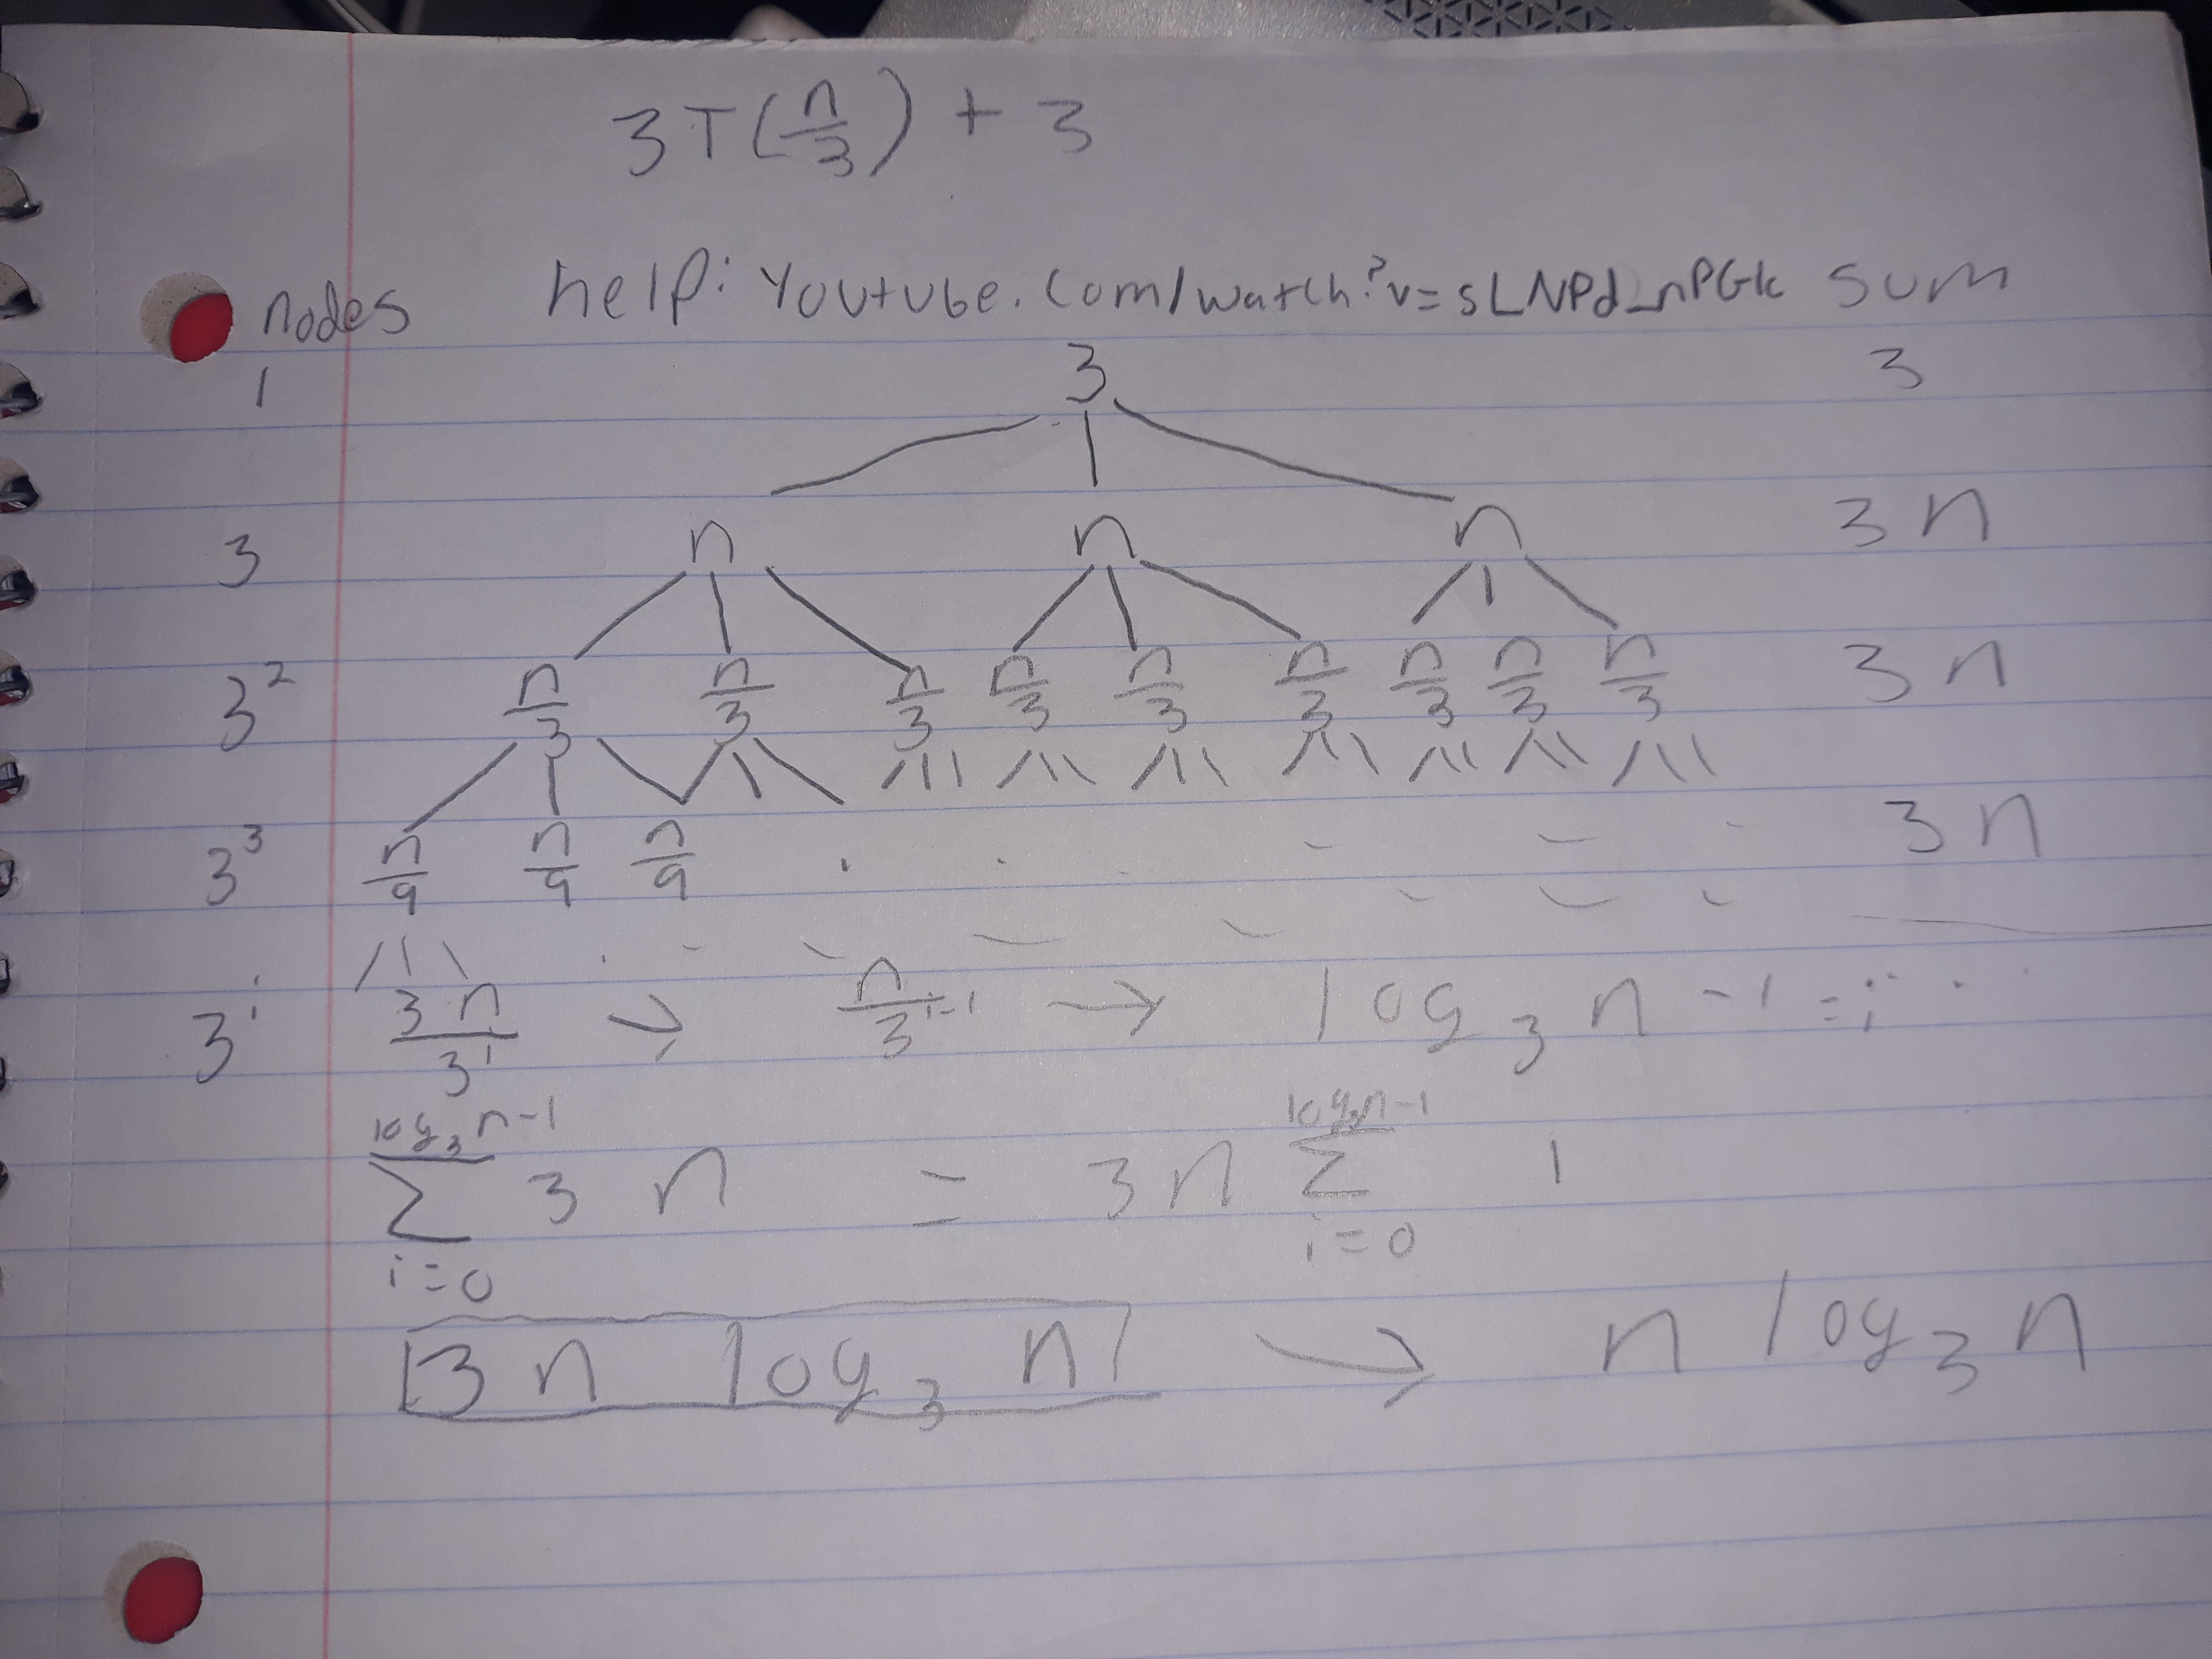
\includegraphics[width=\textwidth]{Tree3} \newline \newline$$\newline$ $T(n)=\Theta(n log_3(n))$
\end{solution}
\pagebreak

\item (4 pts) Give a tight bound ($\Theta$ bound) on the number of {\tt return} calls this algorithm makes. Justify your answer.
\begin{solution}
$\newline$ Return calls occur once every recursive step. Since the array lasts 1 to n (or 0 to (n-1) really, but for us counting, that is 1 to n being counted). All values need to be checked for minimum status, so there is a return every value, making for n returns no matter worst case or best case. $\newline \newline$ Therefore, T(n)=$\Theta(n)$ 
\end{solution}
\end{enumerate}
%\pagebreak


%\makenonemptybox{5in}{}



\pagebreak
\item {\itshape (7 pts) Consider the following algorithm that sorts an array.

\noindent Express and provide the worst-case runtime complexity of this algorithm as a function of $n$, where $n$ represents the size of the array. Provide a tight bound on the worst-case runtime complexity.
}
\begin{verbatim}
buffSort(A, size):
    if size <= 1:
        return
    
    buffSort(A, size-1)
    
    foo = Arr[size-1]
    
    for(index = size-2; index >= 0 AND A[index] > foo; index--)
        A[index+1] = A[index]
    
    A[index+1] = foo
\end{verbatim}

\begin{solution}
$\newline \newline$ T(0)=c $\newline$ a=1, as there is one recursive call to buffSort. $\newline$ t(n)=T(n-1)+n+2 $\newline T(n)=[T(n-2)+(n-1)+2]+n+2 --> T(n)=T(n-2)+n+(n-1)+4 \newline  T(n)=[T(n-3)+(n-2)+2]+n + (n-1) +4 --> T(n-3)+n+(n-1)+(n-2)+6 \newline T(n)=T(n-n)+\sum_{k=0}^{n} n-k +2n --> c+\frac{n}{2}(n+1) + 2n \newline T(n)=c+\frac{1}{2}n^2 + \frac{1}{2}n + 2n --> c+\frac{1}{2}n^2+\frac{5}{2}n \newline \newline$ The highest value is $\frac{1}{2} n^2$, which we can ignore the front on. $\newline \Theta(n^2)$
\end{solution}


\end{enumerate}

\end{document}


